\documentclass[t]{beamer}
%\documentclass[finnish,english,handout]{beamer}

\usepackage[T1]{fontenc}
\usepackage[utf8]{inputenc}
\usepackage{newtxtext} % times
%\usepackage[scaled=.95]{cabin} % sans serif
\usepackage{amsmath}
\usepackage[varqu,varl]{inconsolata} % typewriter
\usepackage[varg]{newtxmath}
\usefonttheme[onlymath]{serif} % beamer font theme
\usepackage{microtype}
\usepackage{epic,epsfig}
\usepackage{amsmath,amsfonts,amssymb}
\usepackage{inputenc}
\usepackage{afterpage}
\usepackage{url}
\urlstyle{same}
\usepackage{amsbsy}
\usepackage{eucal}
\usepackage{rotating}
\usepackage{subcaption}
\usepackage{listings}
\usepackage{lstbayes}
\usepackage[all,poly,ps,color]{xy}
\usepackage{eurosym}
\usepackage{natbib}
\bibliographystyle{apalike}

\mode<presentation>
{
  \setbeamercovered{invisible}
  \setbeamertemplate{itemize items}[circle]
  \setbeamercolor{frametitle}{bg=white,fg=navyblue}
  \setbeamertemplate{navigation symbols}{}
  \setbeamertemplate{headline}[default]{}
  \setbeamertemplate{footline}[split]
  % \setbeamertemplate{headline}[text line]{\insertsection}
  % \setbeamertemplate{footline}[frame number]
}

\pdfinfo{            
  /Title      (BDA, Lecture 8) 
  /Author     (Aki Vehtari) % 
  /Keywords   (Bayesian data analysis)
}

\definecolor{forestgreen}{rgb}{0.1333,0.5451,0.1333}
\definecolor{navyblue}{rgb}{0,0,0.5}
\renewcommand{\emph}[1]{\textcolor{navyblue}{#1}}
\definecolor{darkgreen}{rgb}{0,0.3922,0}

%%%%%%%%%%%%%%%%%%% for hiding figures %%%%%%%%%%%%%%%%%%%%%%%%%%
\usepackage{color}
\newcommand{\hide}[5][white]{
	% usage: \hhide[color]{vspace,hspace,height,width}
	% note: all measures are relative units measured in \textwidth
	%\begin{minipage}{0.99\textwidth}
	\vspace{#2\textwidth}
	\hspace{#3\textwidth}
	\textcolor{#1}{  \rule{#5\textwidth}{#4\textwidth}  }
	% \end{minipage}
      }

\graphicspath{{./figs/}}

\parindent=0pt
\parskip=8pt
\tolerance=9000
\abovedisplayshortskip=2pt

\def\o{{\mathbf o}}
\def\t{{\mathbf \theta}}
\def\w{{\mathbf w}}
\def\x{{\mathbf x}}
\def\y{{\mathbf y}}
\def\z{{\mathbf z}}

\def\peff{p_{\mathrm{eff}}}
\def\eff{\mathrm{eff}}

\DeclareMathOperator{\E}{E}
\DeclareMathOperator{\Var}{Var}
\DeclareMathOperator{\var}{var}
\DeclareMathOperator{\Sd}{Sd}
\DeclareMathOperator{\sd}{sd}
\DeclareMathOperator{\Gammad}{Gamma}
\DeclareMathOperator{\Invgamma}{Inv-gamma}
\DeclareMathOperator{\Bin}{Bin}
\DeclareMathOperator{\Negbin}{Neg-bin}
\DeclareMathOperator{\Poisson}{Poisson}
\DeclareMathOperator{\Beta}{Beta}
\DeclareMathOperator{\logit}{logit}
\DeclareMathOperator{\N}{N}
\DeclareMathOperator{\normal}{normal}
\DeclareMathOperator{\U}{U}
\DeclareMathOperator{\BF}{BF}
\DeclareMathOperator{\Invchi2}{Inv-\chi^2}
\DeclareMathOperator{\NInvchi2}{N-Inv-\chi^2}
\DeclareMathOperator{\InvWishart}{Inv-Wishart}
\DeclareMathOperator{\tr}{tr}
% \DeclareMathOperator{\Pr}{Pr}
\def\euro{{\footnotesize \EUR\, }}
\DeclareMathOperator{\rep}{\mathrm{rep}}

\title[]{Bayesian data analysis}
\subtitle{}

\author{Aki Vehtari}

\institute[Aalto]{}

\begin{document}

\begin{frame}{Chapter 6}

  \begin{itemize}
  \item 6.1 The place of model checking in applied Bayesian statistics
  \item 6.2 Do the inferences from the model make sense?
  \item 6.3 Posterior predictive checking
  \item {\color{gray} 6.4 Graphical posterior predictive checks}    
    \begin{itemize}
    \item[-] this can be skimmed, see instead the paper\\ Gabry et al. (2019). \href{https://doi.org/10.1111/rssa.12378}{\textit{Visualization in Bayesian workflow}}
  \end{itemize}
\item 6.5 Model checking for the educational testing example
  \end{itemize}
  
\end{frame}

\begin{frame}
  
  {\Large\color{navyblue} Model checking}

  \begin{itemize}
  \item demo6\_1: Posterior predictive checking - light speed
  \item demo6\_2: Posterior predictive checking - sequential dependence
  \item demo6\_3: Posterior predictive checking - poor test statistic
  \item demo6\_4: Posterior predictive checking - marginal predictive p-value
  \end{itemize}

\end{frame}

 \begin{frame}{Model checking -- overview}

  \begin{itemize}
  \item<+-> Sensibility with respect to additional information not used in modeling
    \begin{itemize}
    \item e.g., if posterior would claim that hazardous chemical
      decreases probability of death
    \end{itemize}
  \item<+-> External validation
    \begin{itemize}
    \item compare predictions to completely new observations
    \item cf. relativity theory predictions
    \end{itemize}
  \item<+-> Internal validation
    \begin{itemize}
    \item posterior predictive checking
    \item cross-validation predictive checking
    \end{itemize}
  \end{itemize}

\end{frame}

\begin{frame}
  
  {\large\color{navyblue} Simon Newcomb's light of speed experiment in 1882}

  {\small
  Newcomb measured ($n=66$) the time required for light to travel from
  his laboratory on the Potomac River to a mirror at the base of the
  Washington Monument and back, a total distance of 7422 meters.}
  % \begin{center}
  %   \vspace{-0.5\baselineskip}
  %   {\includegraphics[width=7.5cm]{newcomb_data.pdf}}
  % \end{center}

\end{frame}

\begin{frame}{Posterior predictive checking -- example}

  \begin{itemize}
  \item<1-> Newcomb's speed of light measurements 
    \begin{itemize}
    \item model $y\sim\normal(\mu,\sigma)$ with prior $(\mu,\log\sigma)\propto 1$
    \end{itemize}
  \item<2-> Posterior predictive replicate $y^{\rm rep}$
    \begin{itemize}
    \item<3-> draw $\mu^{(s)},\sigma^{(s)}$ from the posterior $p(\mu,\sigma|y)$
    \item<4-> draw $y^{\mathrm{rep}\,(s)}$ from $\normal(\mu^{(s)},\sigma^{(s)})$
    \item<5-> repeat $n$ times to get $y^{\mathrm{rep}}$ with $n$ replicates\\~\\
    \uncover<6->{\includegraphics[width=7cm]{light_ppc_1hist.pdf}}
      \end{itemize}
    \end{itemize}

\end{frame}

\begin{frame}{Replicates vs. future observation}

  \begin{itemize}
  \item Predictive $\tilde{y}$ is the next not yet observed possible
    observation. $y^{\mathrm{rep}}$ refers to replicating the whole
    experiment (potentially with same values of $x$) and obtaining as
    many replicated observations as in the original data.
  \end{itemize}

\end{frame}

\begin{frame}{Posterior predictive checking -- example}

  \begin{itemize}
  \item<1-> Generate several replicated datasets $y^{\rm rep}$
  \item<2-> Compare to the original dataset
  \end{itemize}
  \vspace{-1\baselineskip}
  \uncover<3->{\includegraphics[width=11.5cm]{light_ppc_10hist.pdf}}

\end{frame}

\begin{frame}{Posterior predictive checking -- bayesplot}

  \vspace{-1\baselineskip}
  \texttt{ppc\_hist(y, yrep[1:8,])}
  
  \includegraphics[height=8cm]{Newcomb_ppc_hist.pdf}

\end{frame}

\begin{frame}{Posterior predictive checking -- bayesplot}

  \vspace{-1\baselineskip}
  \texttt{ppc\_dens\_overlay(y, yrep[1:100,])}
  
  \includegraphics[height=8cm]{Newcomb_ppc_dens_overlay.pdf}

\end{frame}

\begin{frame}{Posterior predictive checking -- bayesplot}

  \vspace{-1\baselineskip}
  \texttt{ppc\_ecdf\_overlay(y, yrep[1:100,])}
  
  \includegraphics[height=8cm]{Newcomb_ppc_ecdf_overlay.pdf}

\end{frame}

\begin{frame}{Posterior predictive checking -- bayesplot}

  \vspace{-1\baselineskip}
  \texttt{ppc\_scatter(y, yrep[1:4,]) + geom\_abline()}
  
  \includegraphics[height=7.5cm]{Newcomb_ppc_scatter.pdf}

\end{frame}

\begin{frame}{Posterior predictive checking with test statistic}

  \begin{itemize}
  \item Replicated data sets $y^{\rep}$
  \item Test quantity (or discrepancy measure) $T(y,\theta)$
    \begin{itemize}
    \item summary quantity for the observed data $T(y,\theta)$
    \item summary quantity for a replicated data $T(y^{\rep},\theta)$
    \item can be easier to compare summary quantities than data sets
    \end{itemize}
  \end{itemize}

\end{frame}

\begin{frame}{Posterior predictive checking -- example}

  \begin{itemize}
  \item<1-> Compute test statistic for data $T(y,\theta)=\min(y)$
  \item<2-> Compute test statistic $\min(y^{\rm rep})$ for many replicated datasets 
  \end{itemize}
  \vspace{-1.5\baselineskip}
  \uncover<3->{\includegraphics[width=11cm]{light_ppc_min.pdf}}

\end{frame}

\begin{frame}{Posterior predictive checking -- example}

  \begin{itemize}
  \item<1-> Good test statistic is ancillary (or almost)
    \begin{itemize}
    \item ancillary if it depends only on observed data and if its
      distribution is independent of the parameters of the model
    \end{itemize}
  \item<2-> Bad test statistic is highly dependent of the parameters
    \begin{itemize}
    \item e.g. variance for normal model
    \end{itemize}
  \end{itemize}
  \vspace{-1.5\baselineskip}
  \uncover<3->{\includegraphics[width=10cm]{light_ppc_var.pdf}}

\end{frame}

\begin{frame}{Posterior predictive checking}

  \begin{itemize}
    \only<1->{\color{gray}}
  \item<1-> \textit{Posterior predictive $p$-value}
    \begin{eqnarray*}
      p & = & \Pr(T(y^{\rep},\theta)\geq T(y,\theta)|y)\\
      & = & \int\int
      I_{T(y^{\rep},\theta)\geq T(y,\theta)}p(y^{\rep}|\theta)p(\theta|y)dy^{\rep}d\theta
    \end{eqnarray*}
    where $I$ is an indicator function
    \begin{itemize}
    \item<1-> \only<1->{\color{gray}} having $(y^{\rep\,(s)},\theta^{(s)})$ from the posterior predictive
      distribution, easy to compute
      \begin{equation*}
        T(y^{\rep (s)},\theta^{(s)})\geq T(y,\theta^{(s)}), \quad s=1,\ldots,S
      \end{equation*}
    \end{itemize}
    \vspace{-1.5\baselineskip}
  \item<1-> Posterior predictive $p$-value (ppp-value) estimates whether
    difference between the model and data could arise by chance
  \item<1-> \color{black} Not commonly used, as
    \begin{itemize}
    \item not calibrated in case of non-ancillary statistic
    \item the distribution of test statistic has more information
    \end{itemize}
  \end{itemize}

\end{frame}

\begin{frame}{Posterior predictive checking -- bayesplot}

  \vspace{-1\baselineskip}
  \texttt{ppc\_stat(y, yrep)}, the default statistic "mean" is usually bad
  
  \includegraphics[height=8cm]{Newcomb_ppc_stat_mean.pdf}

\end{frame}

\begin{frame}{Posterior predictive checking -- bayesplot}

  \vspace{-1\baselineskip}
  \texttt{ppc\_stat(y, yrep, stat="min")}
  
  \includegraphics[height=8cm]{Newcomb_ppc_stat_min.pdf}

\end{frame}

\begin{frame}{Posterior predictive checking -- bayesplot}

  \vspace{-1\baselineskip}
  \texttt{ppc\_stat(y, yrep, stat="max")}
  
  \includegraphics[height=8cm]{Newcomb_ppc_stat_max.pdf}

\end{frame}

\begin{frame}{Posterior predictive checking -- bayesplot}

  \vspace{-1\baselineskip}
  \texttt{ppc\_stat2d(y, yrep, stat=c("min","max"))}
  
  \includegraphics[height=8cm]{Newcomb_ppc_stat2d_minmax.pdf}

\end{frame}


% \begin{frame}{Posterior predictive checking -- example}

%   \begin{itemize}
%   \item In general it is often better to improve the model than remove
%     data
%   \item There can be cases where after the first model fit, it is
%     clear that some data are clearly incorrectly measured, but there
%     has to be really strong justifications for dropping out
%     observations
%   \item<2-> Let's assume that in Newcomb experiment, the two observations
%     with negative values are clearly incorrect and let's refit by
%     removing them
%   \end{itemize}

% \end{frame}

  
% \begin{frame}{Posterior predictive checking (good fit)}

%   \vspace{-1\baselineskip}
%   \texttt{ppc\_hist(y2, y2rep[1:8,])}
  
%   \includegraphics[height=8cm]{Newcomb_ppc_hist_nooutliers.pdf}

% \end{frame}

% \begin{frame}{Posterior predictive checking (good fit)}

%   \vspace{-1\baselineskip}
%   \texttt{ppc\_dens\_overlay(y2, y2rep[1:100,])}
  
%   \includegraphics[height=8cm]{Newcomb_ppc_dens_overlay_nooutliers.pdf}

% \end{frame}

% \begin{frame}{Posterior predictive checking (good fit)}

%   \vspace{-1\baselineskip}
%   \texttt{ppc\_ecdf\_overlay(y2, y2rep[1:100,])}
  
%   \includegraphics[height=8cm]{Newcomb_ppc_ecdf_overlay_nooutliers.pdf}

% \end{frame}

% \begin{frame}{Posterior predictive checking (good fit)}

%   \vspace{-1\baselineskip}
%   \texttt{ppc\_stat2d(y2, y2rep, stat=c("min","max"))}
  
%   \includegraphics[height=8cm]{Newcomb_ppc_stat2d_minmax_nooutliers.pdf}

% \end{frame}

% \begin{frame}

%   {\Large\color{navyblue} Calibration of ppp-values}

%   \begin{itemize}
%   \item In the special case that the parameters $\theta$ are known (or
%     estimated to a very high precision) or in which the test statistic
%     $T(y)$ is ancillary (that is,
%     if it depends only on observed data and if its distribution is
%     independent of the parameters of the model) with a continuous
%     distribution, the posterior predictive $p$-value
%     $\Pr(T(y^{\rep})\!>\!T(y)|y)$ has a distribution that is uniform
%     if the model is true.
%   \item Under these conditions, $p$-values less than 0.1 occur 10\% of
%     the time, $p$-values less than 0.05 occur 5\% of the time, and so
%     forth.
%   \end{itemize}

% \end{frame}

% \begin{frame}{Marginal and CV predictive checking}

%   \begin{itemize}
%   \item Consider marginal predictive distributions $p(\tilde{y}_i|y)$
%     and each observation separately
%     \begin{itemize}
%     \item marginal posterior p-values
%       \begin{align*}
%         p_i = \mbox{Pr}(T(y_i^{\rep}) \leq T(y_i) | y)
%       \end{align*}
%       if $T(y_i)=y_i$
%       \begin{align*}
%         p_i = \mbox{Pr}(y_i^{\rep} \leq y_i | y)
%       \end{align*}
%     \end{itemize}
%   \item<2-> if $Pr(\tilde{y}_i|y)$ well calibrated, distribution of $p_i$
%     would be uniform between 0 and 1
%     \begin{itemize}
%     \item holds better for cross-validation predictive tests
%       (cross-validation BDA3 Ch 7) 
%     \end{itemize}
%   \end{itemize}

% \end{frame}

% \begin{frame}{Marginal predictive checking (good fit)}

%   \vspace{-0.5\baselineskip}
%   \begin{itemize}
%   \item Marginal tail area or Probability integral transform (PIT)
%     \begin{align*}
%       p_i = p(y_i^{\rep} \leq y_i | y)
%     \end{align*}
%   \item if $p(\tilde{y}_i|y)$ is well calibrated, distribution of $p_i$'s
%     would be uniform between 0 and 1
%   \end{itemize}
%   \vspace{-1\baselineskip}
%   \only<2>{\includegraphics[width=9.5cm]{Newcomb_PIT_hist.pdf}}
%   \only<3>{\includegraphics[width=9.5cm]{Newcomb_PIT_ecdf.pdf}}
%   \only<4>{\includegraphics[width=9.5cm]{Newcomb_PIT_ecdf_nooutliers.pdf}}


% \end{frame}

\begin{frame}{Example: Exposure to air pollution}

  \begin{itemize}
  \item Example from Jonah Gabry, Daniel Simpson, Aki Vehtari, Michael
    Betancourt, and Andrew Gelman (2019). Visualization in Bayesian
    workflow. \url{https://doi.org/10.1111/rssa.12378}
  \item Estimation of human exposure to air pollution from particulate
    matter measuring less than 2.5 microns in diameter ($\mathrm{PM}_{2.5}$)
    \begin{itemize}
    \item Exposure to $\mathrm{PM}_{2.5}$ is linked to a number of
      poor health outcomes and a recent report estimated that
      $\mathrm{PM}_{2.5}$ is responsible for three million deaths
      worldwide each year (Shaddick et al., 2017)
    \item In order to estimate the public health effect of ambient
      $\mathrm{PM}_{2.5}$, we need a good estimate of the
      $\mathrm{PM}_{2.5}$ concentration at the same spatial resolution
      as our population estimates.
    \end{itemize}
\end{itemize}

\end{frame}

\begin{frame}{Example: Exposure to air pollution}

  \begin{itemize}
  \item Direct measurements of PM 2.5 from ground monitors at 2980
    locations
  \item High-resolution satellite data of aerosol optical depth
    
  \end{itemize}
  \begin{center}
    \only<1>{\vspace{-1.8\baselineskip}\includegraphics[height=7cm]{map-data.png}}
    \only<2>{\vspace{-1.8\baselineskip}\includegraphics[height=7cm]{plot1.png}}
    \only<3>{\hspace{-3cm}\includegraphics[height=6.55cm]{plot2.png}}
\end{center}
\end{frame}

\begin{frame}{Example: Exposure to air pollution}

  Prior predictive checking
  \vspace{-1\baselineskip}
  \begin{center}
    \only<1>{\includegraphics[width=11cm]{pm25_pp1a.pdf}}
    \only<2>{\includegraphics[width=11cm]{pm25_pp1b.pdf}}
    \only<3>{\includegraphics[width=11cm]{pm25_pp2.pdf}}
\end{center}
\end{frame}

\begin{frame}{Example: Exposure to air pollution}

  Posterior predictive checking -- marginal predictive distributions
\begin{figure}
\centering
\begin{subfigure}{0.48\textwidth}
\includegraphics[width=\textwidth]{ppc_dens1.png}
\caption{Model 1}
\end{subfigure}
~
\begin{subfigure}{0.48\textwidth}
\includegraphics[width=\textwidth]{ppc_dens2.png}
\caption{Model 2}
\end{subfigure}
% ~
% \begin{subfigure}{0.31\textwidth}
% \includegraphics[width=\textwidth]{ppc_dens3.png}
% \caption{Model 3}
% \end{subfigure}
\end{figure}

\end{frame}

\begin{frame}{Example: Exposure to air pollution}


  Posterior predictive checking -- test statistic (skewness)
\begin{figure}
\centering
\begin{subfigure}{0.31\textwidth}
\includegraphics[width=\textwidth]{ppc_skew1.png}
\caption{Model 1}
\end{subfigure}
~
\begin{subfigure}{0.31\textwidth}
\includegraphics[width=\textwidth]{ppc_skew2.png}
\caption{Model 2}
\end{subfigure}
~
\begin{subfigure}{0.31\textwidth}
\includegraphics[width=\textwidth]{ppc_skew3.png}
\caption{Model 3}
\end{subfigure}

\end{figure}

\end{frame}

\begin{frame}{Example: Exposure to air pollution}


  Posterior predictive checking -- test statistic (median for groups)

  \begin{figure}
\centering
\begin{subfigure}{.31\textwidth}
\includegraphics[width=\textwidth]{ppc_med_grouped1.png}
\caption{Model 1}
\end{subfigure}
~
\begin{subfigure}{.31\textwidth}
\includegraphics[width=\textwidth]{ppc_med_grouped2.png}
\caption{Model 2}
\end{subfigure}
~
\begin{subfigure}{.31\textwidth}
\includegraphics[width=\textwidth]{ppc_med_grouped3.png}
\caption{Model 3}
\end{subfigure}

\end{figure}

\end{frame}

\begin{frame}{Positive target}
  
    \includegraphics[width=11cm]{mesquite_ppc.pdf}\\
  \vspace{-0.1\baselineskip} {Predicting the yields of mesquite bushes.\\
    \color{gray} \footnotesize
    Gelman, Hill \& Vehtari (2020): Regression and Other Stories, Chapter 11.}\\

\end{frame}

\begin{frame}[fragile]{Student retention}

  Latent hierarchical linear + spline

{\footnotesize
\begin{lstlisting}
nstudents | trials(nstudents1) ~ (assignment | year) +
  s(assignment, k=4), family=binomial()
\end{lstlisting}}

  Latent functions + posterior uncertainty
  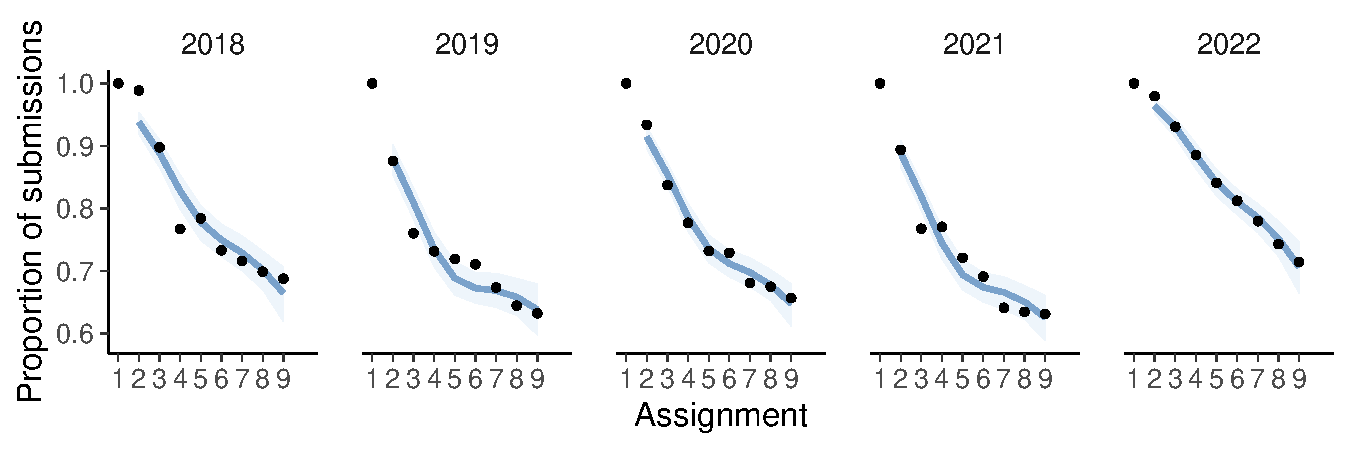
\includegraphics[height=3.6cm]{student_retention_sbinom_linpreds.pdf}
  
\end{frame}

\begin{frame}[fragile]{Student retention}

1. Latent hierarchical linear model
{\footnotesize
\begin{lstlisting}
nstudents | trials(nstudents1) ~ (assignment | year),
  family=binomial()
\end{lstlisting}}

2. Latent hierarchical linear model + spline
{\footnotesize
\begin{lstlisting}
nstudents | trials(nstudents1) ~ (assignment | year) +
  s(assignment, k=4), family=binomial()
\end{lstlisting}}
  
\end{frame}

\begin{frame}[fragile]{Student retention -- Posterior predictive distributions}
\framesubtitle{with \texttt{tidybayes}}
  
\vspace{-0.75\baselineskip}  
Latent hierarchical linear model\\  
  \hspace{-7mm}
  \begin{minipage}[t][3.6cm][t]{1.0\linewidth}
    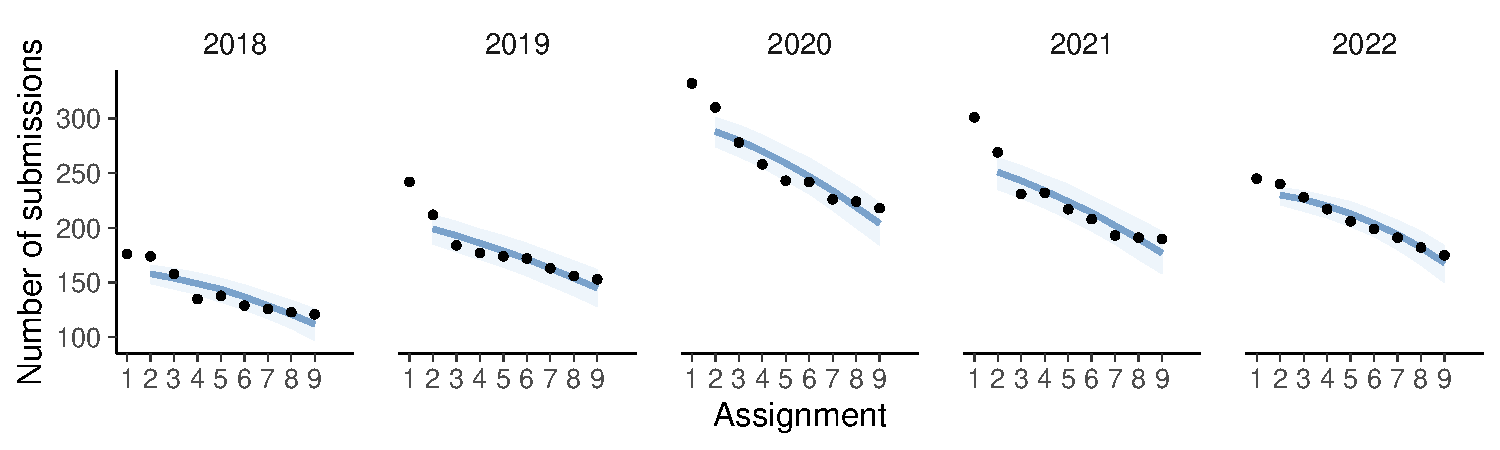
\includegraphics[height=3.6cm]{student_retention_lbinom_preds.pdf}
  \end{minipage}
  
\vspace{-0.25\baselineskip}  
Latent hierarchical linear model + spline\\  
  \hspace{-7mm}
  \begin{minipage}[t][3.6cm][t]{1.0\linewidth}
  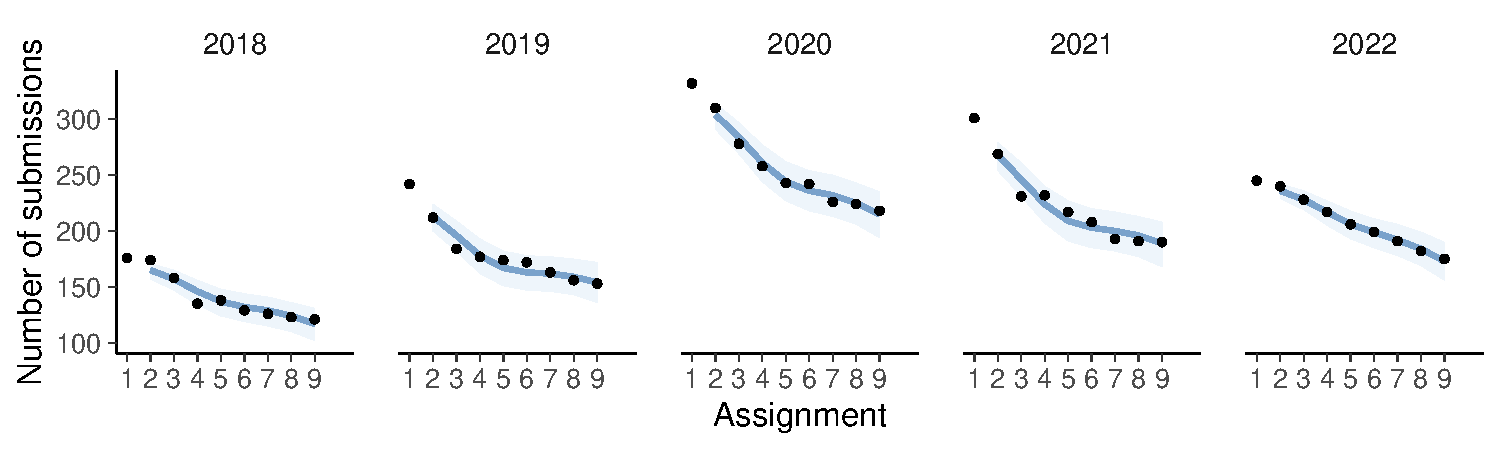
\includegraphics[height=3.6cm]{student_retention_sbinom_preds.pdf}
  \end{minipage}  

\end{frame}

\begin{frame}[fragile]{Student retention -- Marginal PPC}
\framesubtitle{\texttt{pp\_check(fit, ndraws=100)}}

  
\vspace{-0.75\baselineskip}  
Latent hierarchical linear model\\  
  \begin{minipage}[t][3.6cm][t]{1.0\linewidth}
    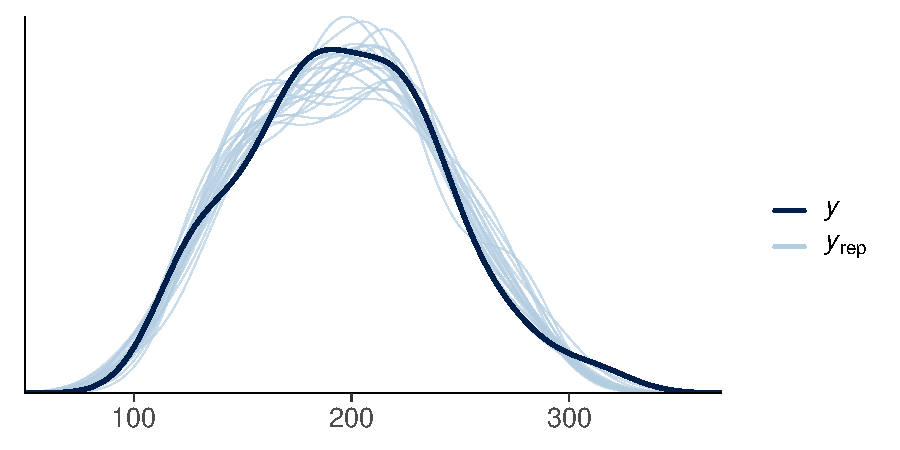
\includegraphics[height=3.6cm]{student_retention_lbinom_ppc_dens_overlay.pdf}
  \end{minipage}
  
\vspace{-0.5\baselineskip}  
Latent hierarchical linear model + spline\\  
  \begin{minipage}[t][3.6cm][t]{1.0\linewidth}
    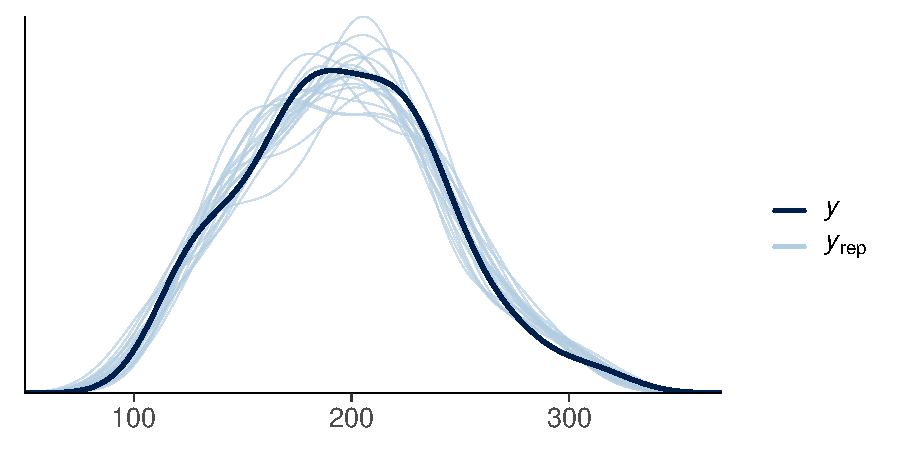
\includegraphics[height=3.6cm]{student_retention_sbinom_ppc_dens_overlay.pdf}
  \end{minipage}  

\end{frame}

\begin{frame}[fragile]{Student retention -- Posterior predictive intervals}
\framesubtitle{\texttt{pp\_check(fit, type = "intervals\_grouped", group="year")}}

\vspace{-0.8\baselineskip}  
Latent hierarchical linear model\\  
  \hspace{-7mm}
  \begin{minipage}[t][3.6cm][t]{1.0\linewidth}
    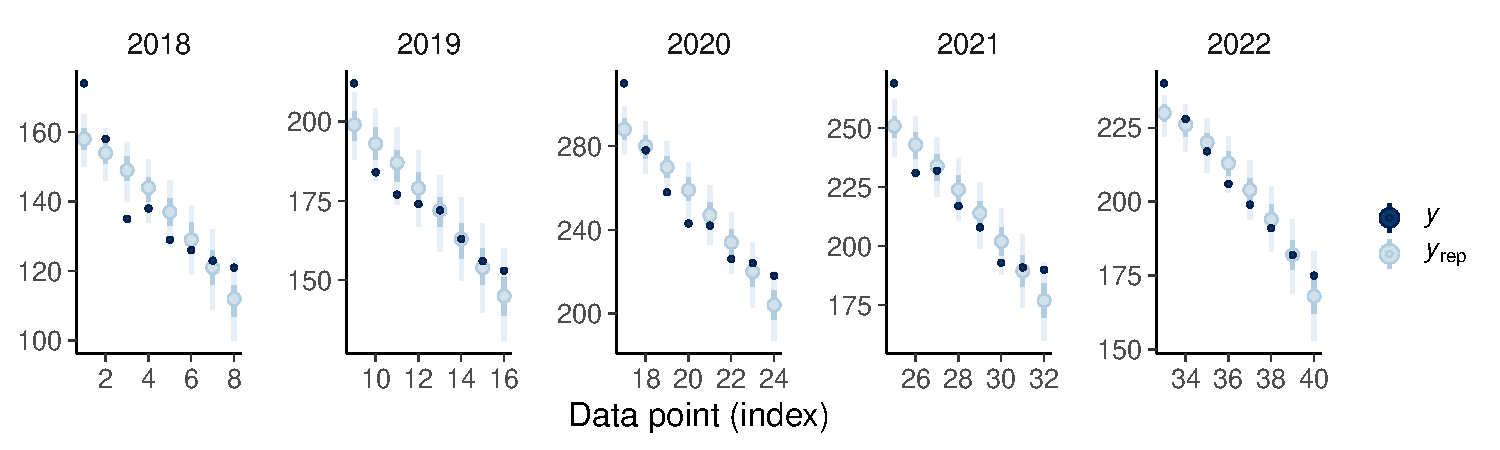
\includegraphics[height=3.6cm]{student_retention_lbinom_ppc_intervals_grouped.pdf}
  \end{minipage}
  
\vspace{-0.5\baselineskip}  
Latent hierarchical linear model + spline\\  
  \hspace{-7mm}
  \begin{minipage}[t][3.6cm][t]{1.0\linewidth}
    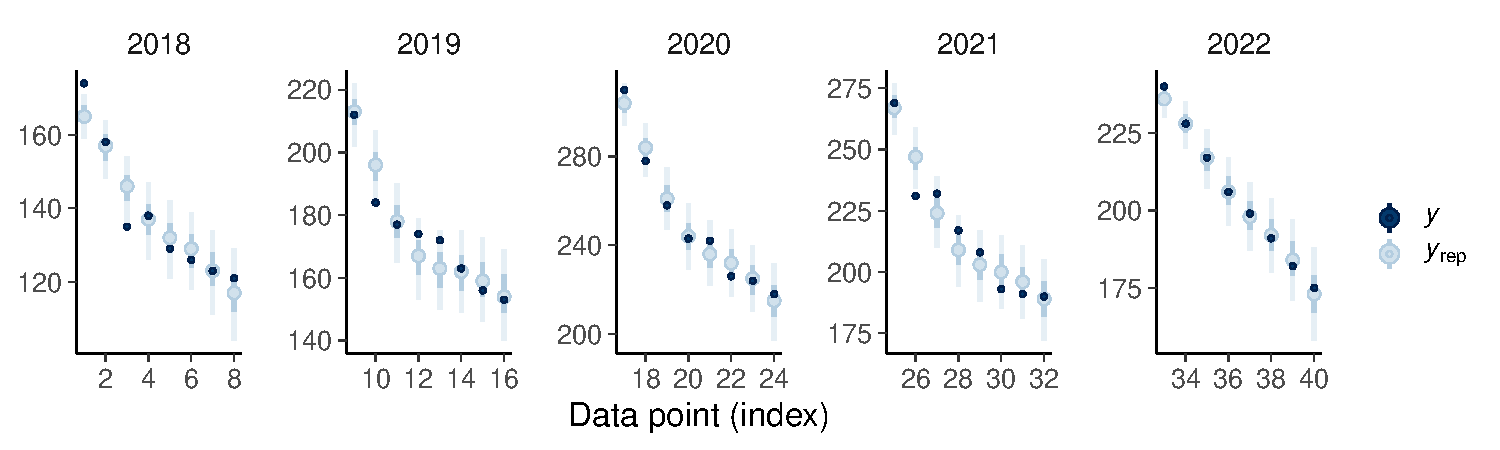
\includegraphics[height=3.6cm]{student_retention_sbinom_ppc_intervals_grouped.pdf}
  \end{minipage}  

\end{frame}

\begin{frame}[fragile]{Student retention -- Posterior predictive ribbon}
\framesubtitle{\texttt{pp\_check(fit, type = "ribbon\_grouped", group="year")}}

\vspace{-0.8\baselineskip}  
Latent hierarchical linear model\\  
  \hspace{-7mm}
  \begin{minipage}[t][3.6cm][t]{1.0\linewidth}
    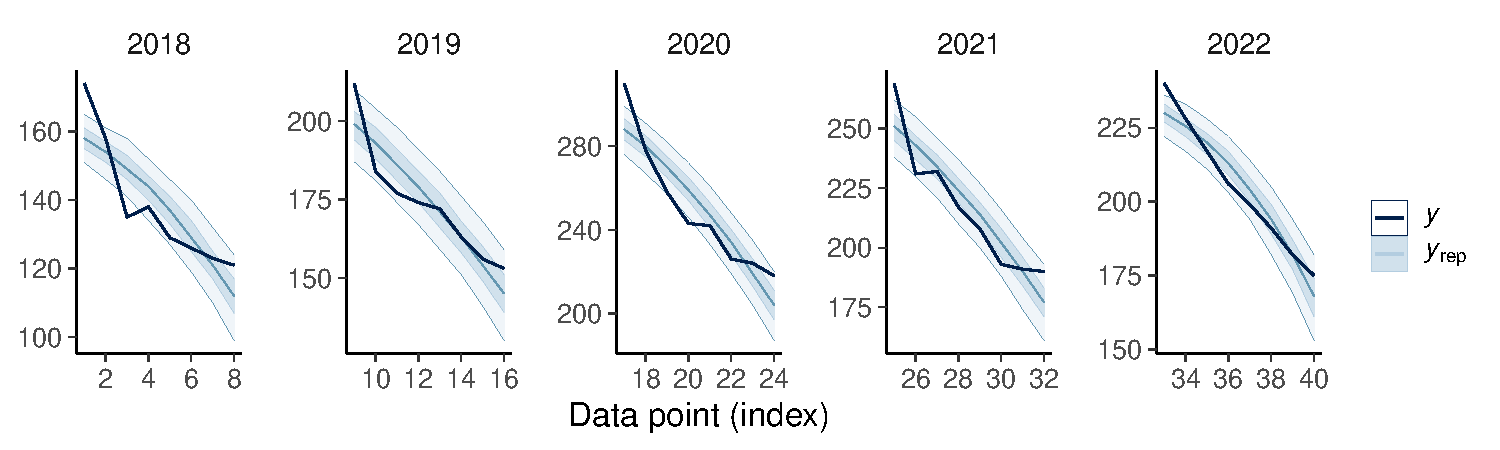
\includegraphics[height=3.6cm]{student_retention_lbinom_ppc_ribbon_grouped.pdf}
  \end{minipage}
  
\vspace{-0.5\baselineskip}  
Latent hierarchical linear model + spline\\  
  \hspace{-7mm}
  \begin{minipage}[t][3.6cm][t]{1.0\linewidth}
    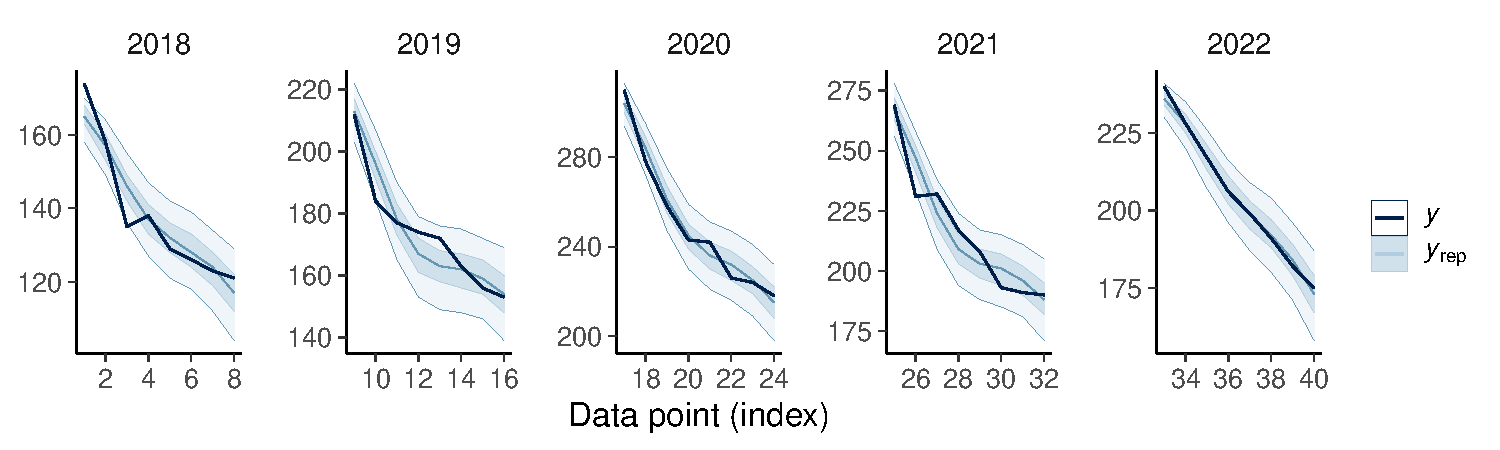
\includegraphics[height=3.6cm]{student_retention_sbinom_ppc_ribbon_grouped.pdf}
  \end{minipage}  

\end{frame}

% \begin{frame}{PPC for binary target}

%   \vspace{-0.75\baselineskip}
%   Diabetes prediction with logistic regression -
%   \href{https://avehtari.github.io/modelselection/diabetes.html}{diabetes demo}
  
%      \only<1>{\vspace{-.6\baselineskip}\includegraphics[width=8.5cm]{diabetes_corrplot.pdf}}
%      \only<2>{PPC with binning for binary data\\ \includegraphics[width=11cm]{diabetes_calibration_binned.pdf}}
%      % \only<3>{PPC with non-linear regression for binary data\\ \includegraphics[width=11cm]{diabetes_calibration_regression.pdf}}
%      \only<3>{PPC with monotonic regression for binary data\\ \includegraphics[width=11cm]{diabetes_reliabilitydiag.pdf}}

% \end{frame}

\begin{frame}[fragile]{PPC for binary target -- Helicopters}

  \vspace{-0.6\baselineskip}
{\scriptsize
\begin{lstlisting}
stable_flight ~ s(wing_length) + s(wing_length, by = nclips),
family = bernoulli()
\end{lstlisting}}
  \vspace{-0.5\baselineskip}
  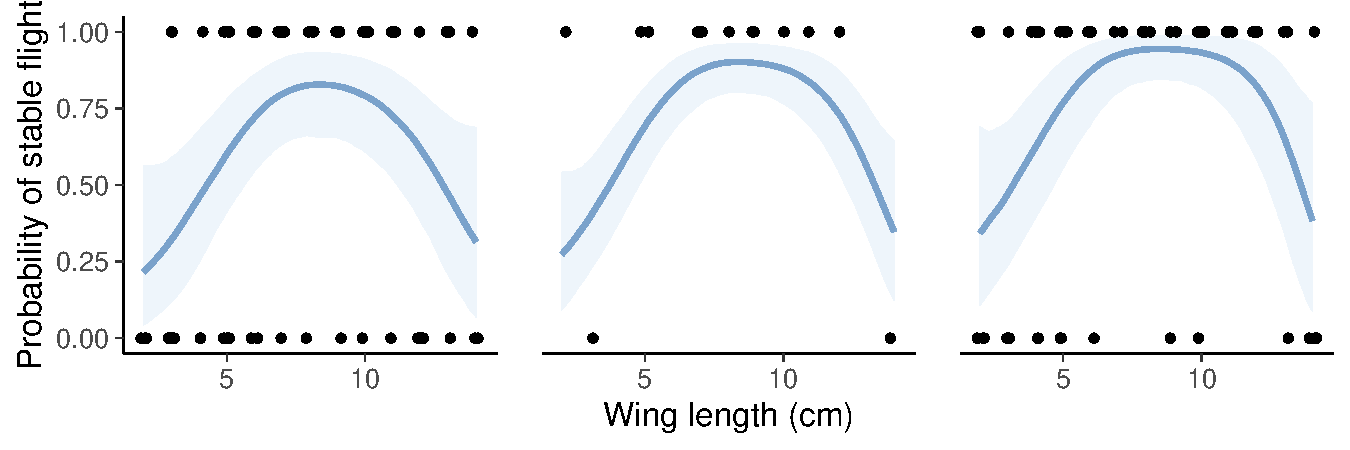
\includegraphics[height=3.6cm]{helicopter_hier_stable.pdf}
  \vspace{-0.1\baselineskip}
  \only<2>{\texttt{pp\_check(fit, ndraws=20)}\\
    \includegraphics[height=3.6cm]{helicopter_hier_stable_ppc_dens_overlay.pdf}}
  \only<3>{\texttt{pp\_check(fit, type="bars")}\\
    \includegraphics[height=3.6cm]{helicopter_hier_stable_ppc_bars.pdf}}
  \only<4>{\texttt{pp\_check(fit, type="bars\_grouped")}\\
    \includegraphics[height=3.6cm]{helicopter_hier_stable_ppc_bars_grouped.pdf}}
  \only<5>{with \texttt{caret::calibration()}\\
    \includegraphics[height=3.6cm]{helicopter_hier_stable_calibration.pdf}}
  \only<6>{with \texttt{reliabilitydiag::reliabilitydiag()}\\
    \includegraphics[height=3.6cm]{helicopter_hier_stable_reliabilitydiag.pdf}}
  
\end{frame}


  
\begin{frame}[fragile]
  \frametitle{Posterior predictive checking -- Stan code}

  \vspace{-0.2\parskip}
  \begin{itemize}
  \item demo demos\_rstan/ppc/poisson-ppc.Rmd
  \end{itemize}

  \vspace{-0.2\parskip}
  {\color{gray}\footnotesize
\begin{lstlisting}[language=Stan]
data {
  int<lower=1> N;
  int<lower=0> y[N];
}
parameters {
  real<lower=0> lambda;
}
model {
  lambda ~ exponential(0.2);
  y ~ poisson(lambda);
}
\end{lstlisting}
  }
  \vspace{-\parskip}
  {\footnotesize
\begin{lstlisting}[language=Stan]
generated quantities {
  real log_lik[N];
  int y_rep[N];
  for (n in 1:N) {
    y_rep[n] = poisson_rng(lambda);
    log_lik[n] = poisson_lpmf(y[n] | lambda);
    }
}
\end{lstlisting}
 }
\end{frame}

\begin{frame}{PPC for count data -- Poisson model}
  
  \vspace{-1\baselineskip}
  \texttt{ppc\_dens\_overlay(y, yrep[1:50,])}

    \includegraphics[height=8cm]{poisson_ppc_dens_overlay.pdf}

\end{frame}

\begin{frame}{PPC for count data -- Poisson model}
  
  \vspace{-1\baselineskip}
  \texttt{ppc\_rootogram(y, yrep)}

    \includegraphics[height=8cm]{poisson_ppc_rootogram.pdf}

\end{frame}

\begin{frame}{PPC for count data -- Poisson model}
  
  \vspace{-1\baselineskip}
  \texttt{prop\_zero <- function(x) mean(x == 0)}\\
  \texttt{ppc\_stat(y, yrep, stat = "prop\_zero")}

    \includegraphics[height=7.5cm]{poisson_ppc_stat_propzero.pdf}

\end{frame}

\begin{frame}{PPC for count data -- hurdle truncated Poisson model}
  
  \vspace{-1\baselineskip}
  \texttt{ppc\_rootogram(y, yrep2)}

    \includegraphics[height=8cm]{poisson2_ppc_rootogram.pdf}

\end{frame}

\begin{frame}{PPC for count data -- hurdle truncated Poisson model}
  
  \vspace{-1\baselineskip}
  \texttt{prop\_zero <- function(x) mean(x == 0)}\\
  \texttt{ppc\_stat(y, yrep2, stat = "prop\_zero")}

    \includegraphics[height=7.5cm]{poisson2_ppc_stat_propzero.pdf}

\end{frame}

\begin{frame}{Further reading and examples}

  \begin{itemize}
  \item Gabry, Simpson, Vehtari, Betancourt, and Gelman
    (2019). Visualization in Bayesian
    workflow. \url{https://doi.org/10.1111/rssa.12378}.
  \item Graphical posterior predictive checks using the bayesplot package
    \url{http://mc-stan.org/bayesplot/articles/graphical-ppcs.html}
  \item Another demo \href{http://avehtari.github.io/BDA_R_demos/demos_rstan/ppc/poisson-ppc.html}{demos\_rstan/ppc/poisson-ppc.Rmd}
  \end{itemize}
  
\end{frame}

\begin{frame}{Sensitivity analysis}

  \begin{itemize}
  \item How much different choices in model structure and priors affect the results
    \begin{itemize}
    \item<2-> test different models and priors\\
      \texttt{priorsense} and \texttt{adjustr} packages use importance
      sampling for faster prior sensitivity analysis
      \item<3-> alternatively combine different models to one model
        \begin{itemize}
        \item e.g. hierarchical model instead of separate and pooled
        \item e.g. $t$ distribution contains Gaussian as a special case
      \end{itemize}
      \item<3-> robust models are good for testing sensitivity to ``outliers''
        \begin{itemize}
        \item e.g. $t$ instead of Gaussian
        \end{itemize}
    \end{itemize}
    \item<4-> Compare sensitivity of essential inference quantities
      \begin{itemize}
      \item extreme quantiles are more sensitive than means and medians
      \item extrapolation is more sensitive than interpolation
      \end{itemize}
    \end{itemize}

\end{frame}

\end{document}

%%% Local Variables: 
%%% TeX-PDF-mode: t
%%% TeX-master: t
%%% End: 
